\chapter{Dataset}
\label{chap:math}
We first had to find a suitable dataset to evaluate the scientific question.
We needed a news dataset that would suffice these requirements:
\begin{itemize}
    \item Contains content of the article for each sample.
    \item Partially contains category, authors, publication date and a publishing server.
    \item Size of at least 200k samples.
    \item Czech language.
\end{itemize}
The closest to our requirements we found were:
\begin{itemize}
    \item \parencite{strakaSumeCzechLargeCzech2018a} - 1M Czech news articles.

          While sufficiently large and in the correct language,
          it contains neither category nor author metadata.
          However, the paper provides valuable information about dataset extraction
          and cleaning of the dataset.
    \item \parencite{misraNewsCategoryDataset2022} - 210k English news articles.

          While it contains both category and author metadata,
          the language is English and the dataset doesn't
          have the content of the articles.
\end{itemize}
As neither dataset suited our needs, we created a new dataset.

\section{Dataset creation}
\label{sec:dataset-creation}

\subsection{Data source}
We initially decided to collect the data from these news servers:
\begin{itemize}
    \item SeznamZprávy.cz
    \item iRozhlas.cz
    \item Novinky.cz
    \item Deník.cz
    \item iDnes.cz
    \item Aktuálně.cz
    \item iHNed.cz
\end{itemize}
We chose these sources due to their popularity and high amount of articles.
To get articles, we had two options:
\begin{enumerate}
    \item Use a web spider to crawl the live website.
    \item Use a web archive that contains crawled articles.
\end{enumerate}
We chose the second option because crawling live websites is tricky,
as the servers would be too fast to block the crawler, due to too many requests. Another advantage of the second approach is that we may not be able to get as many articles as
with a web crawler, since there might be no links to old articles anymore.

\subsection{Webarchive}
As a web archive, we chose a \ac{cc}~\footnote{\url{https://commoncrawl.org/}}.
\ac{cc} is an open-source project crawling the web and storing the data.
The data are stored as a WARC\footnote{\url{https://www.iso.org/obp/ui/\#iso:std:iso:28500:ed-2:v1:en}} files in \ac{s3}.
The data can be queried using Amazon's big data tools or \ac{cc} API.
\ac{cc} data has been collected since 2008 with various frequencies,
since 2014 they have been collected monthly.

\subsection{Data extraction}
\subsubsection{CC Extractor}
To extract the data, we developed a utility \textbf{\ac{cmc}} that can extract the data from a \ac{cc}
based on the URL, crawl date, etc\dots. \ac{cmc} was
created, strongly emphasizing scalability and reliability, as a huge amount of data
was required to be processed.

It's separated into two parts:
\begin{enumerate}
    \item \ac{cag} -
          Extracts links from \ac{cc} API for specified URLs and sends them to a Processor.
    \item \ac{cap} -
          Loads the WARC data from \ac{s3} and extracts the requested metadata.
          We used Python's beautifulsoup\footnote{\url{https://pypi.org/project/beautifulsoup4/}} library for extraction.
\end{enumerate}
Both of them can be scaled based on the needs.
The connection between the \ac{cag} and \ac{cap} can be made using various middlewares.
We used ActiveMQ Artemis~\footnote{\url{https://activemq.apache.org/components/artemis}} for our purposes.
When the \ac{cag} send links to \ac{cap},
they are filtered for uniqueness based on the normalized version(URL without query, deduplicated '\verb|/|' etc\dots).
\subsubsection{Extraction}
We have done extraction on 12.12.2022 on \ac{aic}\footnote{\url{https://aic.ufal.mff.cuni.cz}}.
We set the \ac{cmc} to only output articles in which \ac{cap} successfully
extracted the content and headline.
We set \ac{cmc} to aggregate crawls from 1.1.2008 to 31.8.2022\footnote{
    We limited the choice of crawls. Those crawls contain articles older than 2008,
    which is why the date range of the dataset is bigger.}.
We run one \ac{cag} and four \acp{cap} for each server,
totaling 7 \acp{cag} and 28 \acp{cap}.
As for orchestration, while \ac{cmc} has working docker support,
the cluster doesn't support it, thus we used shell scripts for deployment.
The 49.2M URLs were aggregated, of which 3.2M were successfully extracted.

Once we extracted the data, we started with filtering and postprocessing.
\subsection{Filtering}

Filtering was done in several steps. We employed \ac{hf} datasets\footnote{\url{https://huggingface.co/docs/datasets/index}}
library, as it allows for parallel processing of the data.
This allowed us to filter the data in a few hours on a single machine.


\subsection{iHNed.cz articles}
Similar to~\textcite{strakaSumeCzechLargeCzech2018a}, we found that the iHNed.cz articles contained
a high number of paywalled articles and overall contained few samples.
We thus decided to drop it.

\subsection{Czech filtering}
Since we were interested in Czech articles, we decided to filter out articles
not in the Czech language. For this purpose,
we used FastText Language detection model~\parencites{joulinFastTextZipCompressing2016}{joulinBagTricksEfficient2016}.
For every article, we used the model to predict the language of every line.
This allowed us to interpret fractions of lines predicted as Czech as the confidence of the article being in the Czech language.
We inspected the articles with lower confidence and the most occurring problems were:
\begin{enumerate}
    \item Articles in Ukraine language on SeznamZprávy.cz, due to the recent war in Ukraine.
    \item Articles with a list of sports results, where most texts were.
          the result, team and match highlights.
    \item Articles with comparison tables, e.g., mobile comparison.
    \item Galeries; there were few articles with galleries of pictures or videos with little text.
    \item English articles on iDnes.cz and iRozhlas.cz.
\end{enumerate}
Since we had many articles, we decided to filter out articles with a confidence lower than 1.0.

\subsubsection{Filtering by Article Statistics}
\label{sec:filtering-by-article-statistics}
The main goal of this step was to filter out either wrongly parsed
or non-news articles (plain sports results, weather, tables, videos/photos\dots).
We inspected article content based on several properties
and set the following thresholds to remove unwanted articles:
\begin{enumerate}
    \item General:
          \begin{enumerate}
              \item Content length - $(400, \inf)$
              \item Headline length - $(20, \inf)$
              \item Brief length - $(40, \inf)$
              \item Publication date - $(1.1.2000, 31.8.2022)$
          \end{enumerate}
    \item Content:
          \begin{enumerate}
              \item Average word length - $(4.0, \inf)$
              \item Num of words / Lenght - $(0.11, 0.22)$
              \item Non-alphanumeric characters / Length - $(0, 0.045)$
          \end{enumerate}
\end{enumerate}

During the inspection, we further found the following problems:
\begin{enumerate}
    \item Headline cuts

          When observing articles with short headlines, we found that the headlines
          were cut in the middle of words.
          It was because the extractor had a function that would remove anything after '\verb|-|'.
          In headlines, it was supposed to prevent the bloat like '\verb|- Aktuálně.cz|'. However,
          we didn't anticipate this would also remove words like start-up, n‑tice, etc\dots.
          We removed this rule and reran the whole extraction.
    \item Content character length

          Observing content length at Novinky.cz and SeznamZprávy.cz, we found many articles with content of fewer than 100 characters, due to an extraction error.
          For these two sites, we were extracting content by CSS classes.
          However, we didn't include all possible classes, as they are likely autogenerated;
          thus, sometimes extractor extracted only headers.
          We tried to fix the problems by adding more classes and generalizing the CSS selectors,
          reducing the issue but not eradicating it. We thus decided to resolve this problem
          by the content length rule.

    \item Headline length drops

          When inspecting Aktuálně.cz, we found that the article counts peaked
          at certain headline lengths (55, 60, 85), followed by a steep drop in numbers.
          However, we haven't found any problems with such headlines.
          We assume these inconveniences result from internal rules for writers at Aktuálně.cz.
\end{enumerate}

\subsubsection{filtering by headline content}
As in \textcite{strakaSumeCzechLargeCzech2018a}, many articles
contained prefixes at headlines like '\verb|VIDEO: |', '\verb|FOTO: |', '\verb|GALERIE: |' etc\dots.
Since we were interested in the articles and not galleries,
we dropped the articles with prefixes that indicate non-news content.
However, unlike \textcite{strakaSumeCzechLargeCzech2018a}, we haven't removed these prefixes
in non-filtered headlines/briefs.




\subsubsection{Headline/Brief/Content dedupliation}
The last filtering round removed articles with identical briefs, headlines or content.
We were afraid that this would also affect the article across different servers.
It turned out that the deduplication only deleted around 3k articles
because of cross-server duplicates.
When choosing, which duplicate to use, we took the one with the most metadata filled
or the longer article length.
Therefore, every Brief/Content/Headline is unique in the dataset.

\subsection{Data Augmentation and Postprocessing}

\subsubsection{Category}
\label{sec:category}
Due to the wide variety of collected data, we had to normalize categories.
After extraction, we got a total of 3383 categories.
Since there was considerable overlap between each category,
we selected 25 categories among the most popular ones.
We focused on choosing the categories with the most samples,
while ensuring a slight overlap between selected categories.
That's why we dropped categories like \textit{News, Tips, Your News, Other, etc\dots},
even though they had many samples.
We then mapped from the remaining categories to these 25 categories if such a mapping was possible.
Examples of such mappings are:
\begin{enumerate}
    \item Football, Tennis, Biathlon\dots $\rightarrow$ Sport
    \item Praha, Domažlicko, Ústecko\dots $\rightarrow$ Home
    \item She, Women, Fashion\dots $\rightarrow$ Lifestyle
\end{enumerate}

\subsubsection{Authors}
\label{sec:authors}
After extraction, there were 27k unique authors.
The obvious problem was that not all authors were people.
Surprisingly, the most prevalent were the news institutions: \textit{ČTK, IDnes, MF DNES, etc\dots}.
There were also many nicknames we couldn't decode, companies,
and common names like \textit{Redakce, externí, etc\dots}.

We employed heuristics and manual filtering
to mitigate these problems and ended up with 11K authors.
As for postprocessing, we removed occupation and academic titles.

\subsubsection{Gender and cumulative gender}
\label{sec:gender}
To infer the gender of the author's name, we used Namsor \footnote{\url{https://namsor.app/}}
as suggested by \textcite{seboPerformanceGenderDetection}.
For cumulative gender, we used the following rules:
\begin{enumerate}
    \item If all authors of the article are Man $\rightarrow$ Man.
    \item If all authors of the article are Woman $\rightarrow$ Woman.
    \item Mixed otherwise.
\end{enumerate}

\subsubsection{Content, Brief, Headline Postprocessing}
We used the following postprocessing steps for content, brief and headline:
\begin{enumerate}
    \item Replace '\verb|\n|,\verb|\r|,\verb|\t|' with spaces
    \item Truncate spaces
    \item Convert named and numeric character references to Unicode
    \item Normalize Unicode characters to their base combined form
\end{enumerate}
As for Brief and Headline, we capitalized the first letter
and added a dot at the end if there wasn't one.

\subsection{Splits}
\label{sec:splits}
Since we were interested in predicting the future,
we decided to split the data into train, validation and test set based on the publication date.
The sets are, therefore, not random but ordered by publication date. Train set having the earliest, while test the latest articles.
If the sample didn't have a publication date, we randomly assigned it to one of the sets.
We selected the ratio between splits to \textbf{85:7.5:7.5}.
Due to experiments, we also additionally created the following splits:
\begin{enumerate}
    \item\label{enum:train-small} \textbf{Train Small} - 50K most recent samples from the training set, containing all metadata
    \item\label{enum:test-small} \textbf{Test Small} - 10K randomly selected samples from the test set, containing all metadata
    \item\label{enum:test-human} \textbf{Test Human} - 100 randomly selected samples from test set, containing all metadata
\end{enumerate}

\section{Dataset summary}
\begin{table}[H]
    \resizebox{\linewidth}{!}{%
        \centering\footnotesize\sf
        \begin{tabular}{lrrrrr}
            \toprule
            {}          & Size    & Unique Authors & Categories & Date Range            & Article words \\
            \midrule
            Deník.cz   & 664133  & 2497           & 18         & 27.3.2007 - 6.8.2022  & 332           \\
            Novinky.cz   & 321417  & 2518           & 17         & 20.12.2002 - 6.8.2022 & 274           \\
            iDnes.cz & 295840  & 4385           & 21         & 3.1.2000 - 9.8.2022   & 423           \\
            iRozhlas.cz   & 167588  & 1900           & 8          & 8.7.2000 - 25.6.2022  & 287           \\
            Aktuálně.cz   & 112960  & 633            & 19         & 26.10.2005 - 6.8.2022 & 468           \\
            SeznamZprávy.cz   & 65472   & 382            & 11         & 14.9.2016 - 6.8.2022  & 443           \\
            \midrule
            Total       & 1627410 & 10930          & 25         & 3.1.2000 - 9.8.2022   & 362           \\
            \bottomrule
        \end{tabular}
        \caption{Dataset summary. Article words were calculated based
            on Moses tokenization}
        \label{tab:dataset_summary}
    }
\end{table}
The summarization of the dataset is shown in~\autoref{tab:dataset_summary}.
The dataset contains the following features:
\begin{itemize}
    \item \textbf{Content} - Article content
    \item \textbf{Brief} - Brief/Perex of the article
    \item \textbf{Headline} - Headline/Title of the article
    \item \textbf{Category} - Both post-processed and original category
    \item \textbf{Published Date} - Date of publication and inferred day of week
    \item \textbf{Authors} - Authors, with their textual gender and cumulative gender
    \item \textbf{Keywords} - Extracted keywords from the article
    \item \textbf{Comments Count} - Number of comments in discussion section
\end{itemize}
We further provide a more detailed description of each task in the following sections.
\todo{add numbers}

\subsection{Server}
\label{sec:server-desc}
\begin{figure}[H]
    \centering
    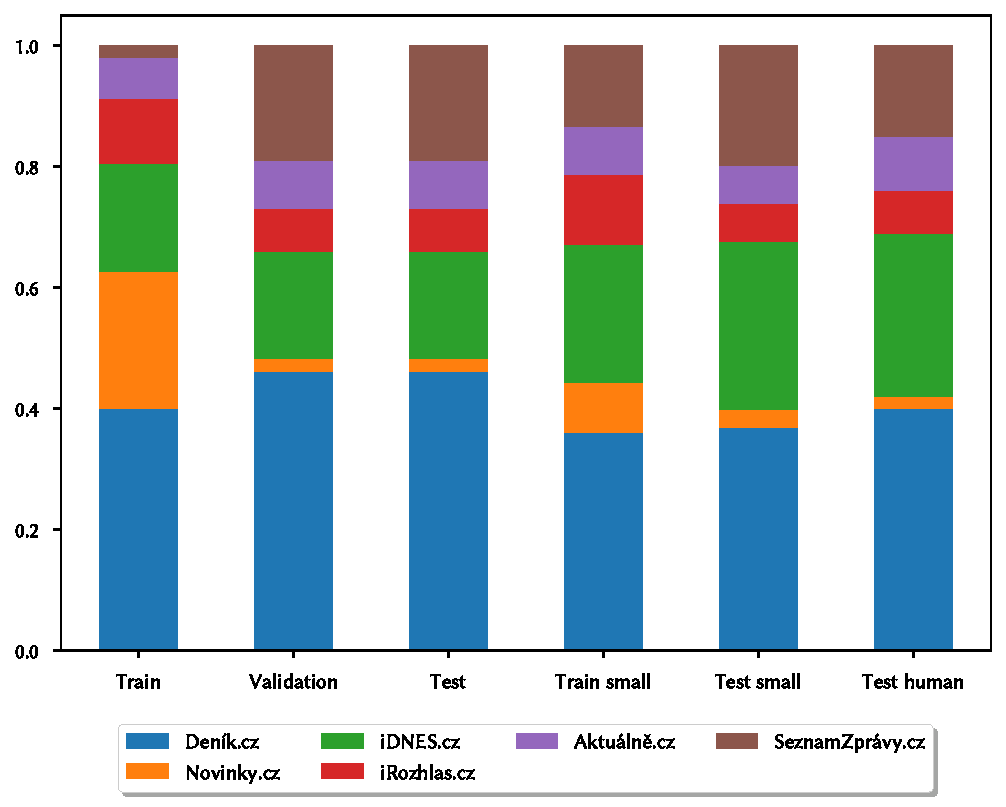
\includegraphics[width=0.9\textwidth]{img/tasks_graph/server.pdf}
    \caption{Graph depicting proportion of servers among the datasets}
    \label{fig:server_graph}
\end{figure}
From~\autoref{fig:server_graph}, we can see that the most frequent server is Deník.cz.
That is due to regional coverage not being present on the other servers. We can also see
a shallow representation of the SeznamZprávy.cz in the training set.
This occurs because the server was launched the latest, among others, in 2016.
The extinction of Novinky.cz in the test and validation set is likely explained by \autoref{sec:filtering-by-article-statistics}.
We can also observe higher proportions of iDnes.cz in subsamples of the test set.
That is because iDnes.cz contains all metadata more often than the other servers.
\todo{CHECK THIS I Assumed it}


\subsection{Category}
\begin{figure}[H]
    \centering
    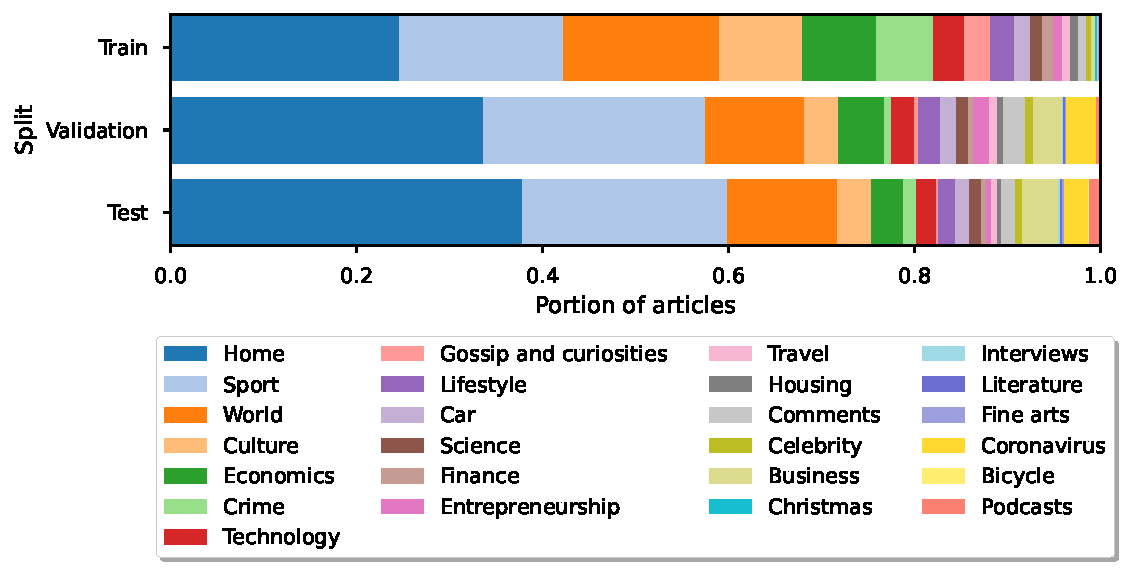
\includegraphics[width=0.9\textwidth]{img/tasks_graph/category.pdf}
    \caption{Graph depicting distribution categories among the datasets}
    \label{fig:category_graph}
\end{figure}
As seen in~\autoref{fig:category_graph}, Home is the most frequent category.
We know it might overlap with other categories like Economy, but we decided to keep it separate.
We didn't wan to drop home as it contains most of the political articles.

\subsection{Day of the Week}
\begin{figure}[H]
    \centering
    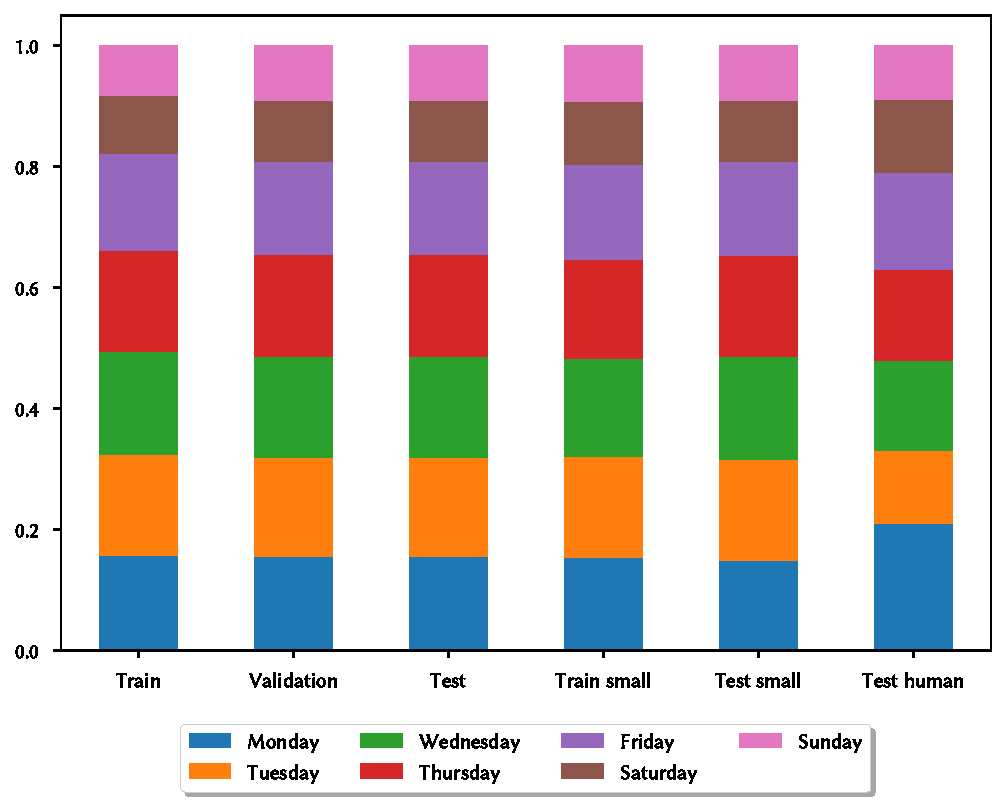
\includegraphics[width=0.9\textwidth]{img/tasks_graph/day_of_week.pdf}
    \caption{Graph depicting the distribution of weekdays among the datasets}
    \label{fig:day_graph}
\end{figure}
The days of the week are evenly distributed among the datasets, as seen in~\autoref{fig:day_graph}.
We can see more articles published on weekdays than on weekends.

\subsection{Gender}
\begin{figure}[H]
    \centering
    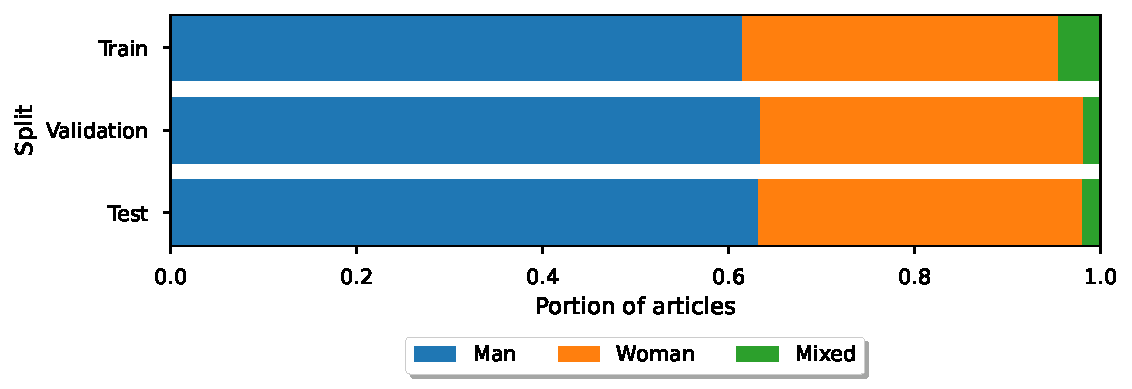
\includegraphics[width=0.9\textwidth]{img/tasks_graph/authors_cum_gender.pdf}
    \caption{Graph depicting the distribution of genders among the datasets}
    \label{fig:gender_graph}
\end{figure}
For the Gender task, we use cumulative gender as described in~\autoref{sec:gender}.
We were surprised that the genders are skewed towards men (around $60\%$) as seen in~\autoref{fig:gender_graph}.
It might be due to Namsor misclassifying female names as male names or there might be a prevalence of male names in the Czech media.